\documentclass{article}
\usepackage[english]{babel}
\usepackage[letterpaper,top=2cm,bottom=2cm,left=3cm,right=3cm,marginparwidth=1.75cm]{geometry}
\usepackage{amsmath}
\usepackage{graphicx}
\usepackage[colorlinks=true, allcolors=blue]{hyperref}

\title{Anonymous provision of services via blockchain}
% Anonymous and fair provision of physical services via blockchain
\author{Stanisław Barański}
\date{December 2021}

\providecommand{\keywords}[1]{\textbf{Keywords:} #1}


\begin{document}
\maketitle

\begin{abstract}
Lorem ipsum\ldots
\end{abstract}
\keywords{data privacy, privacy preserving, blockchain, fair-exchange}



\section{Problem statement}
Service providers (SP) like: lawyers, laboratories, auditors, or banks, to provide services, require data that is often associated with user identity.

Providing personal information exposes users to privacy risk, i.e. potential loss of control over personal information ~\cite{smith2011information}. 

Such user information can be then used deliberately or unintentionally (e.g, by theft) for: insider disclosure, unauthorized access, or commercial gains. For example, by reselling it to marketers, financial institutions, other businesses, government agencies, or even cybercriminals. Which in turn can lead to profiled advertisements, or criminal activities like identity theft or illegal tracking and surveillance~\cite{smith2011information}.

The guarantee of the privacy of the data is based on a trust assumptions and security of IT systems. However, most of the service providers don't need the information of user identity for other reasons than payment, communication, or logistics. 

It would be desirable if the user could keep its identity private, while service provider still provide its services. This could lead to reduced trust that users have to put on SP and less responsibility borne by SP.

In this paper we propose a protocol for anonymous provision of services via blockchain and cryptography techniques. Specificaly, we use
\begin{enumerate}
    \item \textbf{confidential blockchain} to process payment for a service without revealing a user's identity.
    \item \textbf{zero-knowledge proofs} — to proof the payment for the service without revealing the payment itself.
    \item \textbf{encryption scheme and blockchain} — to asynchronously deliver the results of the made service back to the user.
\end{enumerate}


Authors of the paper~\cite{lin2021efficient} propose a system for Privacy-Preserving Credit Score System. Letting banks to calculate creditworthness without learning user private information like registration, hobbies, credit, relationships, and inquiry. To achieve this they use Paillier encryption and noninteractive zero-Knowledge schemes (NIZK).

\subsection{Fair-exchange protocols}

We observe that such protocols for providing services are special case of fair-exchange protocol.

Fair-exchange protocol is a protocol used for performing e-commerce transactions of both digital and physical goods, exchanging documents, or signing contracts, between mutually distrusting parties, while satisfying following conditions:
\begin{itemize}
    \item non-repudiation  — any participating party can not deny their actions (e.g. signing, sending, and receiving data). Usually this is achieved by digital signatures.
    \item fairness — any participating party does not gain any advantage at any step of the exchange protocol.
    \item timeliness — the protocol eventually terminates for all participants.
\end{itemize}

There are two main categories of fair-exchange protocols~\cite{kremer2002intensive,duangphasuk2020fair}: those that involve the use of trusted third party (TTP), and those that do not.

\paragraph{Protocols that do not involve use of trusted third party.}
Protocols that do not involve use of trusted third party, also called "probabilistic" or "gradual" exchange protocols. In such protocols~\cite{markowitch1999probabilistic}, items that will be exchanged are first split into parts. Then, the parts are exchanged between parties. This causes increased communication overhead. Moreover the fairness of such protocol is probabilistic, meaning that there is a small chance that the protocol will end up with one party being in advantageous position. 

Hence, the great benefit of TTP-less protocol, comes at a cost of increased communication overhead, and unsatisfactory property of uncertain termination.


\paragraph{Protocols that involve the use of trusted third party}
The most common approach to achieve fair-exhange conditions is by introducing Trusted Third Party (TTP).  

TTP can play different role in fair-exchange protocol. Commonly agreed classification~\cite{kremer2002intensive,duangphasuk2020fair} distinguish three roles the TTP can play:

\begin{enumerate}
    \item Inline~\cite{coffey1996non}, the TTP act as a authoritative middleman between sender and receiver. The obvious consequence of such method is the communication bottleneck and single point of failure. These protocols are inefficient and trust-dependent.
    
    \item Online~\cite{djuric2015feips}, the TTP is involved in each protocol step, but not in each data transmission. Significantly improving the performance compared to inline TTP.
    
    \item Offline~\cite{hwang2015provable}, the TTP is involved only in case of a dispute between parties. This approach is also called "optimistic", because in scenarios where both parties behaves honesty, the TTP is ignored. Resulting in high-performance and low trust-dependency. 
\end{enumerate}

Involving online and centralized TTP in each transaction, could cause the communication bottleneck problem. Therefore, the offline TTP is the most favorable approach.

The main idea of the offline TTP model is that the sender sends a ciphertext of his/her own document before obtaining the expect document from opposite party. Both parties will then fairly exchange the decryption keys of the ciphertext. 

\section{E-commerce transaction protocol}

According to ~\cite{djuric2015feips}, a typical e-commerce process can be illustrated with the diagram on figure ~\ref{fig:ecommerce-transaction-diagram}.

\begin{figure}[htbp]
\centerline{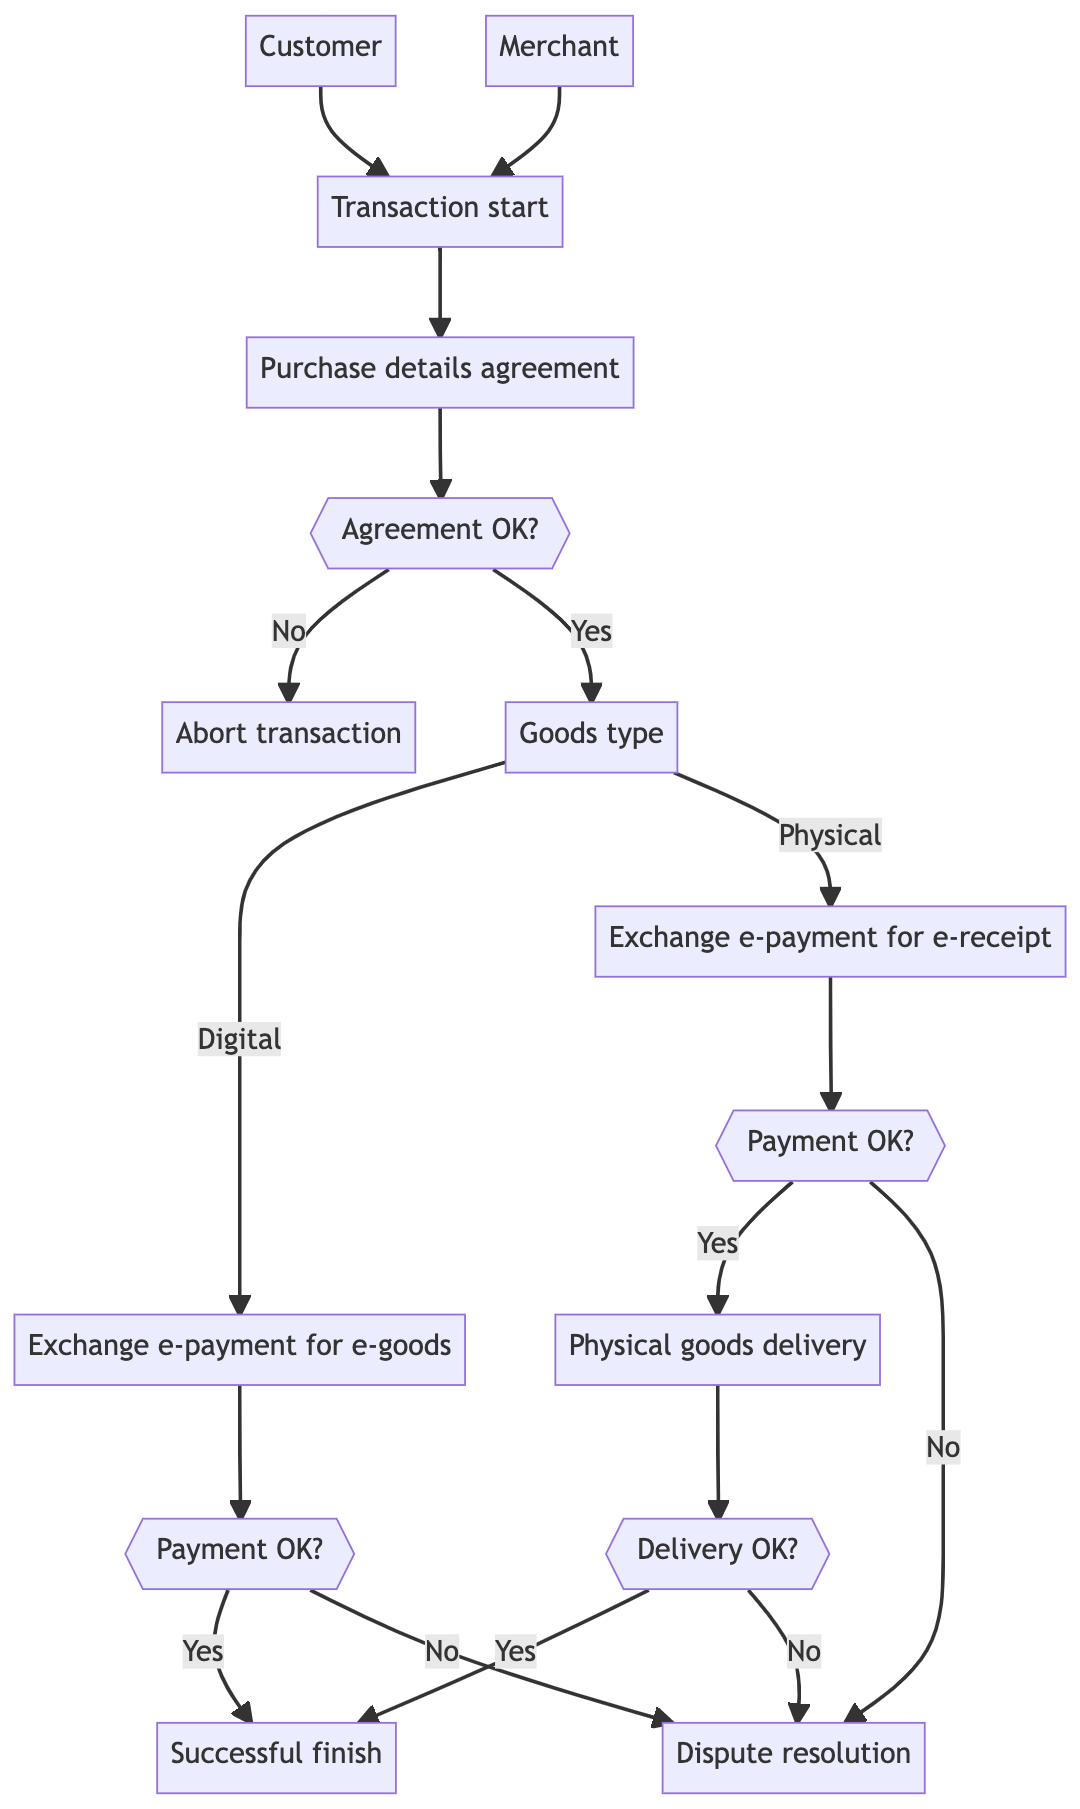
\includegraphics[width=.4\linewidth]{ecommerce-process.png}}
\caption{Diagram illustrating a typical e-commerce transaction process}
\label{fig:ecommerce-transaction-diagram}
\end{figure}


\section{Anonymous fair-exchange}

An protocol ensures anonymity if no party can make a link between identity and actions taken by another party.

\subsection{State of the art}
\subsubsection{Anonymity and fair-exchange in e-commerce protocol for physical products delivery}

Authors of ~\cite{birjoveanu2015anonymity} proposed a fair-exchange of physical product and electronic payment protocol that guarantee both customer and merchant anonymity. They achieve it by introducing online trusted third party that validate coins and provide fair exchange guarantees. 

The anonymity is ensured by assuming the existence of source cabinet (SC) and delivery cabinet (DC), and a trusted delivery agent who take product from a source cabinet and provide it to a destination cabinet. 
Both cabinets provides access to the product by passwords to conceal identity of the customer and the merchant.
To avoid identity disclosure of customer and merchant, the access to the product is provided by passwords. 

Both cabinets are equipment with cameras. Also there should exist the trusted delivery agent (DA) who will deliver items from source cabinet do delivery cabinet. 

The protocol works as follows:
\begingroup
\renewcommand{\labelenumii}{\arabic{enumii}.}
\begin{enumerate}
    \item Both parties agree on the purchase details.
    \item The customer buys a digital coin from his bank and validates it with the TTP.
    \item The customer sends to the merchant the purchase order and the digital signature made by TTP on the encrypted coin.
    \item The merchant post the product to the source cabinet.
    \item Delivery agent collect the product from source cabinet and post it to delivery cabinet.
    \item Customer collects the product from delivery cabinet using password.
    \item The customer checks if the product is actually the ordered one.
    \begin{itemize}
    \item[-] if yes 
        \begin{enumerate}
        \setcounter{enumii}{7}
        \item the customer sends the acknowledge to delivery cabinet and decryption key to the merchant.
        \item The merchant redeem the coins from the bank.
        \end{enumerate}
    \item[-] if no
        \begin{enumerate}
        \setcounter{enumii}{7}
        \item the delivery cabinet is equipment with video camera that records the moment when the customer open the package and let the customer to signal the invalidity of the product, and so, sending the encrypted recording to the TTP. 
        \item the dispute is settled via TTP, optionally letting each party to reveal it's identity.
    \end{enumerate}
    \end{itemize}
\end{enumerate}
\endgroup

Yet, the fair-exchange properties are achieved by strong assumptions. Namely, 
\begin{itemize}
    \item the TTP does not misbehave or collude with any party. 
    \item The customer's and merchant's banks enable confidental transactions and both share commit-buffer where the value is locked until the transaction is finished.   
    \item All banks mantain a global list of coin's serial numbers to prevent double-spending problem. 
    \item The source cabinet and delivery cabinet exists, and in both the product access is protected by password.
    \item Delivery cabinet is equppted with a video camera that records the moment when the customer opens the package, and provide a way to submit the video to TTP in case of a dispute. 
    \item Delivery agent exist and is trusted. 
    \item Communication channels between parties provides anonymity.
\end{itemize}

\subsubsection{Themis} Themis~\cite{meng2019themis} is a fair-exchange protocol, which uses blockchain instead of TTP. It provide escrow services for secure exchanging between cryptocurrencies and physical goods.

Authors highlight that a widely-used atomic exchange mechanism HTLC (Hashed Time-lock Contract) is vulnerable to denial of service (DoS) attacks. While Multi-Signature Schemes depends on the Trusted Third Party (TTP) making them vulnerable to collusion attacks. Such TTP can collude with one party and take the locked funds. It can also refuse settling disputes and lock the hosted funds. 

Themis is a decentralized system which provides an escrow and dispute resolution serivces. It satisfies following requirements:
\begin{description}
    \item[Fairness] Either both seller and buyer obtain all the goods, or they both obtain nothing.
    \item[Security] The funds are locked until the transaction is completed.
    \item[Passivity] If no dispute arise, the third-party does not need to involve in the transaction.
    \item[Correctness] Transactions and disputes are executed according to a priori agreed protocol rules.
    \item[Dependability] There is no single point of failure vulnerable to DoS attack.
    \item[Privacy] If the dispute does not arise, the third-party does not know if the transaction completes. If the dispute arises, only the related parties are aware of it.    
\end{description}

\subsection{A Solution for Secure Certified Electronic Mail Using Blockchain as a Secure Message Board}


\section{Contribution}
In this paper similarly to by~\cite{birjoveanu2015anonymity}, we propose fully-fledged protocol for anonymous fair-exchange which includes payment processing and physical goods exchange. Yet, compared to ~\cite{birjoveanu2015anonymity}, we use decentralized blockchain instead of centralized TTP, and payments using cryptocurrencies, getting rid of strong and unrealistic assumptions on traditional banking.

Additionally, since the services are provided locally, we enable customers to disclose the transaction and start the dispute in law.

Once the package is delivered to the SP, the SP publish POR (Proof-of-recipment) on the blockchain. From this point the customer is secured, i.e. if the merchant misbehaves, customer can proof to the justice that he paid for the service at a particular point of time, and that SP received the package, but didn't publish results. 


Or we can create a smart contract that automatically punish the SP if he doesn't fulfull the agreement in time. And the proof to justice is used in case where the content of the service is invalid, something that have to be settled by human.

If merchant misbehaves i.e. does not provide the agreed services, then the customer can create a proof that such incident happened 
However it provide a proof that such incident happened. In settings where the identity of the party is known, such proof can be used to bring the misbehaving party to the justice.


\section{Applications}
\subsection{Anonymous clinical tests}
Bodybuilders, athletes,  weightlifters, cyclists, football and rugby players have to pass anti-doping tests before attending the competition. 

Patients willing to check steroid tests, drug tests, venereal diseases — anything that they wouldn't want to share with anyone, have to risk that the data stored in laboratory won't get to unauthorized hands like attacker or malicious worker.

Analysis of urine, saliva, stool, or blood. 

\subsection{Anonymous lawyer consultations}

People willing to take business action that may be risky or not yet fully legistlated, may be willing to receive the estimation of risks and repercussions of such action.
Such protocol would provide a mechanism for 


\subsection{Anonymous financial trustworthiness evaluation}

Evaluating financial trustworthiness is required when user want to, for example issue a credit card, take loan for a home, or rent a car. 
As defined in~\cite{lin2021efficient}, such a system consist of three parties: (i) users, (ii) credit bureaus, and (iii) creditors. Users willing to take a credit, have to provide to the credit bureaus, their financial activities like: new account creation, account balance, credit card utilization, credit inquires, and payment history. Such information are then submitted to creditors to compute the user's credit score. 

\subsection{Anonymous physical delivery e-commerce}
% TODO write about
~\cite{birjoveanu2015anonymity}


% [![](https://mermaid.ink/img/eyJjb2RlIjoic2VxdWVuY2VEaWFncmFtXG4gICAgQ3VzdG9tZXItPj5TbWFydCBDb250cmFjdDogUHJvdmlkZSBkZXRhaWxzLCBsb2NrIGZ1bmRzLlxuXHRhY3RpdmF0ZSBTbWFydCBDb250cmFjdFxuXHRTbWFydCBDb250cmFjdCAtPj4gU21hcnQgQ29udHJhY3Q6IENyZWF0ZSBhZ3JlZW1lbnRcblx0ZGVhY3RpdmF0ZSBTbWFydCBDb250cmFjdFxuXHRhbHQgSWYgc2VydmljZSBwcm92aWRlciBkZWNsaW5lIGFncmVlbWVudFxuXHRTZXJ2aWNlIFByb3ZpZGVyIC0-PiBTbWFydCBDb250cmFjdDogRGVjbGluZVxuXHRTbWFydCBDb250cmFjdCAtPj4gQ3VzdG9tZXI6IFJlZnVuZFxuXHRlbmRcblx0U2VydmljZSBQcm92aWRlciAtPj4gU21hcnQgQ29udHJhY3Q6IEFjY2VwdFxuXHRcblx0YWx0IGRpZ2l0YWwgZG9jdW1lbnRzXG5cdFx0cGFyIGF0b21pYyB0cmFuc2FjdGlvblxuXHRcdEN1c3RvbWVyIC0-PiAgb2ZmLWNoYWluIHN0b3JhZ2U6IFB1Ymxpc2ggZW5jcnlwdGVkIGRvY3VtZW50c1xuXHRcdG9mZi1jaGFpbiBzdG9yYWdlIC0tPj4gQ3VzdG9tZXI6IFByb29mLW9mLURlbGl2ZXJ5IChQT0QpXG5cdFx0ZW5kXG5cdEN1c3RvbWVyIC0-PiBTbWFydCBDb250cmFjdDogUHVibGlzaCBQT0Rcblx0ZWxzZSBwaHlzaWNhbCBkb2N1bWVudHNcblx0XHRwYXIgYXRvbWljIHRyYW5zYWN0aW9uXG5cdFx0Q3VzdG9tZXIgLT4-ICBTZXJ2aWNlIFByb3ZpZGVyOiBQcm92aWRlIGRvY3VtZW50cyBwaHlzaWNhbGx5XG5cdFx0U2VydmljZSBQcm92aWRlciAtPj4gU21hcnQgQ29udHJhY3Q6IFB1Ymxpc2ggUE9EXG5cdFx0ZW5kXG5cdGVuZFxuXHRsb29wIGV4ZWN1dGUgdW50aWwgY3VzdG9tZXIgaXMgc2F0aXNmaWVkIHdpdGggcmVzdWx0c1xuXHRTZXJ2aWNlIFByb3ZpZGVyIC0-PiBTZXJ2aWNlIFByb3ZpZGVyOiBFeGVjdXRlIHNlcnZpY2Vcblx0U2VydmljZSBQcm92aWRlciAtPj4gT2ZmLWNoYWluIHN0b3JhZ2U6IFB1Ymxpc2ggZW5jcnlwdGVkIHJlc3VsdHNcblx0U2VydmljZSBQcm92aWRlciAtPj4gU21hcnQgQ29udHJhY3Q6IFB1Ymxpc2ggUHJvb2Ytb2YtUmVzdWx0c1xuXHRcblx0XG5cdEN1c3RvbWVyIC0-PiBTbWFydCBDb250cmFjdDogR2V0IFByb29mLW9mLVJlc3VsdHNcblx0Q3VzdG9tZXIgLT4-IE9mZi1jaGFpbiBzdG9yYWdlOiBHZXQgcmVzdWx0c1xuXHRDdXN0b21lciAtPj4gQ3VzdG9tZXI6IFZhbGlkYXRlIHJlc3VsdHNcblx0YWx0IHJlc3VsdHMgYXJlIGluY29ycmVjdFxuXHRcdEN1c3RvbWVyIC0-PiBTbWFydCBDb250cmFjdDogU3RhcnQgZGlzcHV0ZSwgcHJvdmlkZSBkZXRhaWxzXG5cdFx0YWx0IFNlcnZpY2UgUHJvdmlkZXIgZGVjbGluZSBhcmd1bWVudHNcblx0XHRcdFNtYXJ0IENvbnRyYWN0IC0-PiBTZXJ2aWNlIFByb3ZpZGVyOiBVbmxvY2sgZnVuZHNcblx0XHRcdG5vdGUgcmlnaHQgb2YgU2VydmljZSBQcm92aWRlcjogU1AgaXMgYWx3YXlzIG9uIGxvc3QgcG9zaXRpb24sIDxicj5iZWNhdXNlIGhlIGNhbiBub3Qgc3VlIGFub255bW91cyBjdXN0b21lci48YnI-IFRoZXJlZm9yZSB0aGUgc2hvdWxkIGJlIHRoZSBob2xkZXIgdGhlIGZ1bmRzIGFzIHNvb24gYXMgcG9zc2libGUuXG5cdFx0XHRDdXN0b21lciAtPj4gUG9saWNlOiBPcGVuIGRpc3B1dGUgYXQgcG9saWNlXG5cdFx0ZW5kXG5cdGVuZFxuXHRlbmRcblx0XG5cbiAgICBcbiAgICAgICAgICAgICIsIm1lcm1haWQiOnsidGhlbWUiOiJkZWZhdWx0In0sInVwZGF0ZUVkaXRvciI6ZmFsc2UsImF1dG9TeW5jIjp0cnVlLCJ1cGRhdGVEaWFncmFtIjpmYWxzZX0)](https://mermaid.live/edit#eyJjb2RlIjoic2VxdWVuY2VEaWFncmFtXG4gICAgQ3VzdG9tZXItPj5TbWFydCBDb250cmFjdDogUHJvdmlkZSBkZXRhaWxzLCBsb2NrIGZ1bmRzLlxuXHRhY3RpdmF0ZSBTbWFydCBDb250cmFjdFxuXHRTbWFydCBDb250cmFjdCAtPj4gU21hcnQgQ29udHJhY3Q6IENyZWF0ZSBhZ3JlZW1lbnRcblx0ZGVhY3RpdmF0ZSBTbWFydCBDb250cmFjdFxuXHRhbHQgSWYgc2VydmljZSBwcm92aWRlciBkZWNsaW5lIGFncmVlbWVudFxuXHRTZXJ2aWNlIFByb3ZpZGVyIC0-PiBTbWFydCBDb250cmFjdDogRGVjbGluZVxuXHRTbWFydCBDb250cmFjdCAtPj4gQ3VzdG9tZXI6IFJlZnVuZFxuXHRlbmRcblx0U2VydmljZSBQcm92aWRlciAtPj4gU21hcnQgQ29udHJhY3Q6IEFjY2VwdFxuXHRcblx0YWx0IGRpZ2l0YWwgZG9jdW1lbnRzXG5cdFx0cGFyIGF0b21pYyB0cmFuc2FjdGlvblxuXHRcdEN1c3RvbWVyIC0-PiAgb2ZmLWNoYWluIHN0b3JhZ2U6IFB1Ymxpc2ggZW5jcnlwdGVkIGRvY3VtZW50c1xuXHRcdG9mZi1jaGFpbiBzdG9yYWdlIC0tPj4gQ3VzdG9tZXI6IFByb29mLW9mLURlbGl2ZXJ5IChQT0QpXG5cdFx0ZW5kXG5cdEN1c3RvbWVyIC0-PiBTbWFydCBDb250cmFjdDogUHVibGlzaCBQT0Rcblx0ZWxzZSBwaHlzaWNhbCBkb2N1bWVudHNcblx0XHRwYXIgYXRvbWljIHRyYW5zYWN0aW9uXG5cdFx0Q3VzdG9tZXIgLT4-ICBTZXJ2aWNlIFByb3ZpZGVyOiBQcm92aWRlIGRvY3VtZW50cyBwaHlzaWNhbGx5XG5cdFx0U2VydmljZSBQcm92aWRlciAtPj4gU21hcnQgQ29udHJhY3Q6IFB1Ymxpc2ggUE9EXG5cdFx0ZW5kXG5cdGVuZFxuXHRsb29wIGV4ZWN1dGUgdW50aWwgY3VzdG9tZXIgaXMgc2F0aXNmaWVkIHdpdGggcmVzdWx0c1xuXHRTZXJ2aWNlIFByb3ZpZGVyIC0-PiBTZXJ2aWNlIFByb3ZpZGVyOiBFeGVjdXRlIHNlcnZpY2Vcblx0U2VydmljZSBQcm92aWRlciAtPj4gT2ZmLWNoYWluIHN0b3JhZ2U6IFB1Ymxpc2ggZW5jcnlwdGVkIHJlc3VsdHNcblx0U2VydmljZSBQcm92aWRlciAtPj4gU21hcnQgQ29udHJhY3Q6IFB1Ymxpc2ggUHJvb2Ytb2YtUmVzdWx0c1xuXHRcblx0XG5cdEN1c3RvbWVyIC0-PiBTbWFydCBDb250cmFjdDogR2V0IFByb29mLW9mLVJlc3VsdHNcblx0Q3VzdG9tZXIgLT4-IE9mZi1jaGFpbiBzdG9yYWdlOiBHZXQgcmVzdWx0c1xuXHRDdXN0b21lciAtPj4gQ3VzdG9tZXI6IFZhbGlkYXRlIHJlc3VsdHNcblx0YWx0IHJlc3VsdHMgYXJlIGluY29ycmVjdFxuXHRcdEN1c3RvbWVyIC0-PiBTbWFydCBDb250cmFjdDogU3RhcnQgZGlzcHV0ZSwgcHJvdmlkZSBkZXRhaWxzXG5cdFx0YWx0IFNlcnZpY2UgUHJvdmlkZXIgZGVjbGluZSBhcmd1bWVudHNcblx0XHRcdFNtYXJ0IENvbnRyYWN0IC0-PiBTZXJ2aWNlIFByb3ZpZGVyOiBVbmxvY2sgZnVuZHNcblx0XHRcdG5vdGUgcmlnaHQgb2YgU2VydmljZSBQcm92aWRlcjogU1AgaXMgYWx3YXlzIG9uIGxvc3QgcG9zaXRpb24sIDxicj5iZWNhdXNlIGhlIGNhbiBub3Qgc3VlIGFub255bW91cyBjdXN0b21lci48YnI-IFRoZXJlZm9yZSB0aGUgc2hvdWxkIGJlIHRoZSBob2xkZXIgdGhlIGZ1bmRzIGFzIHNvb24gYXMgcG9zc2libGUuXG5cdFx0XHRDdXN0b21lciAtPj4gUG9saWNlOiBPcGVuIGRpc3B1dGUgYXQgcG9saWNlXG5cdFx0ZW5kXG5cdGVuZFxuXHRlbmRcblx0XG5cbiAgICBcbiAgICAgICAgICAgICIsIm1lcm1haWQiOiJ7XG4gIFwidGhlbWVcIjogXCJkZWZhdWx0XCJcbn0iLCJ1cGRhdGVFZGl0b3IiOmZhbHNlLCJhdXRvU3luYyI6dHJ1ZSwidXBkYXRlRGlhZ3JhbSI6ZmFsc2V9)
\begin{figure}[htbp]
\centerline{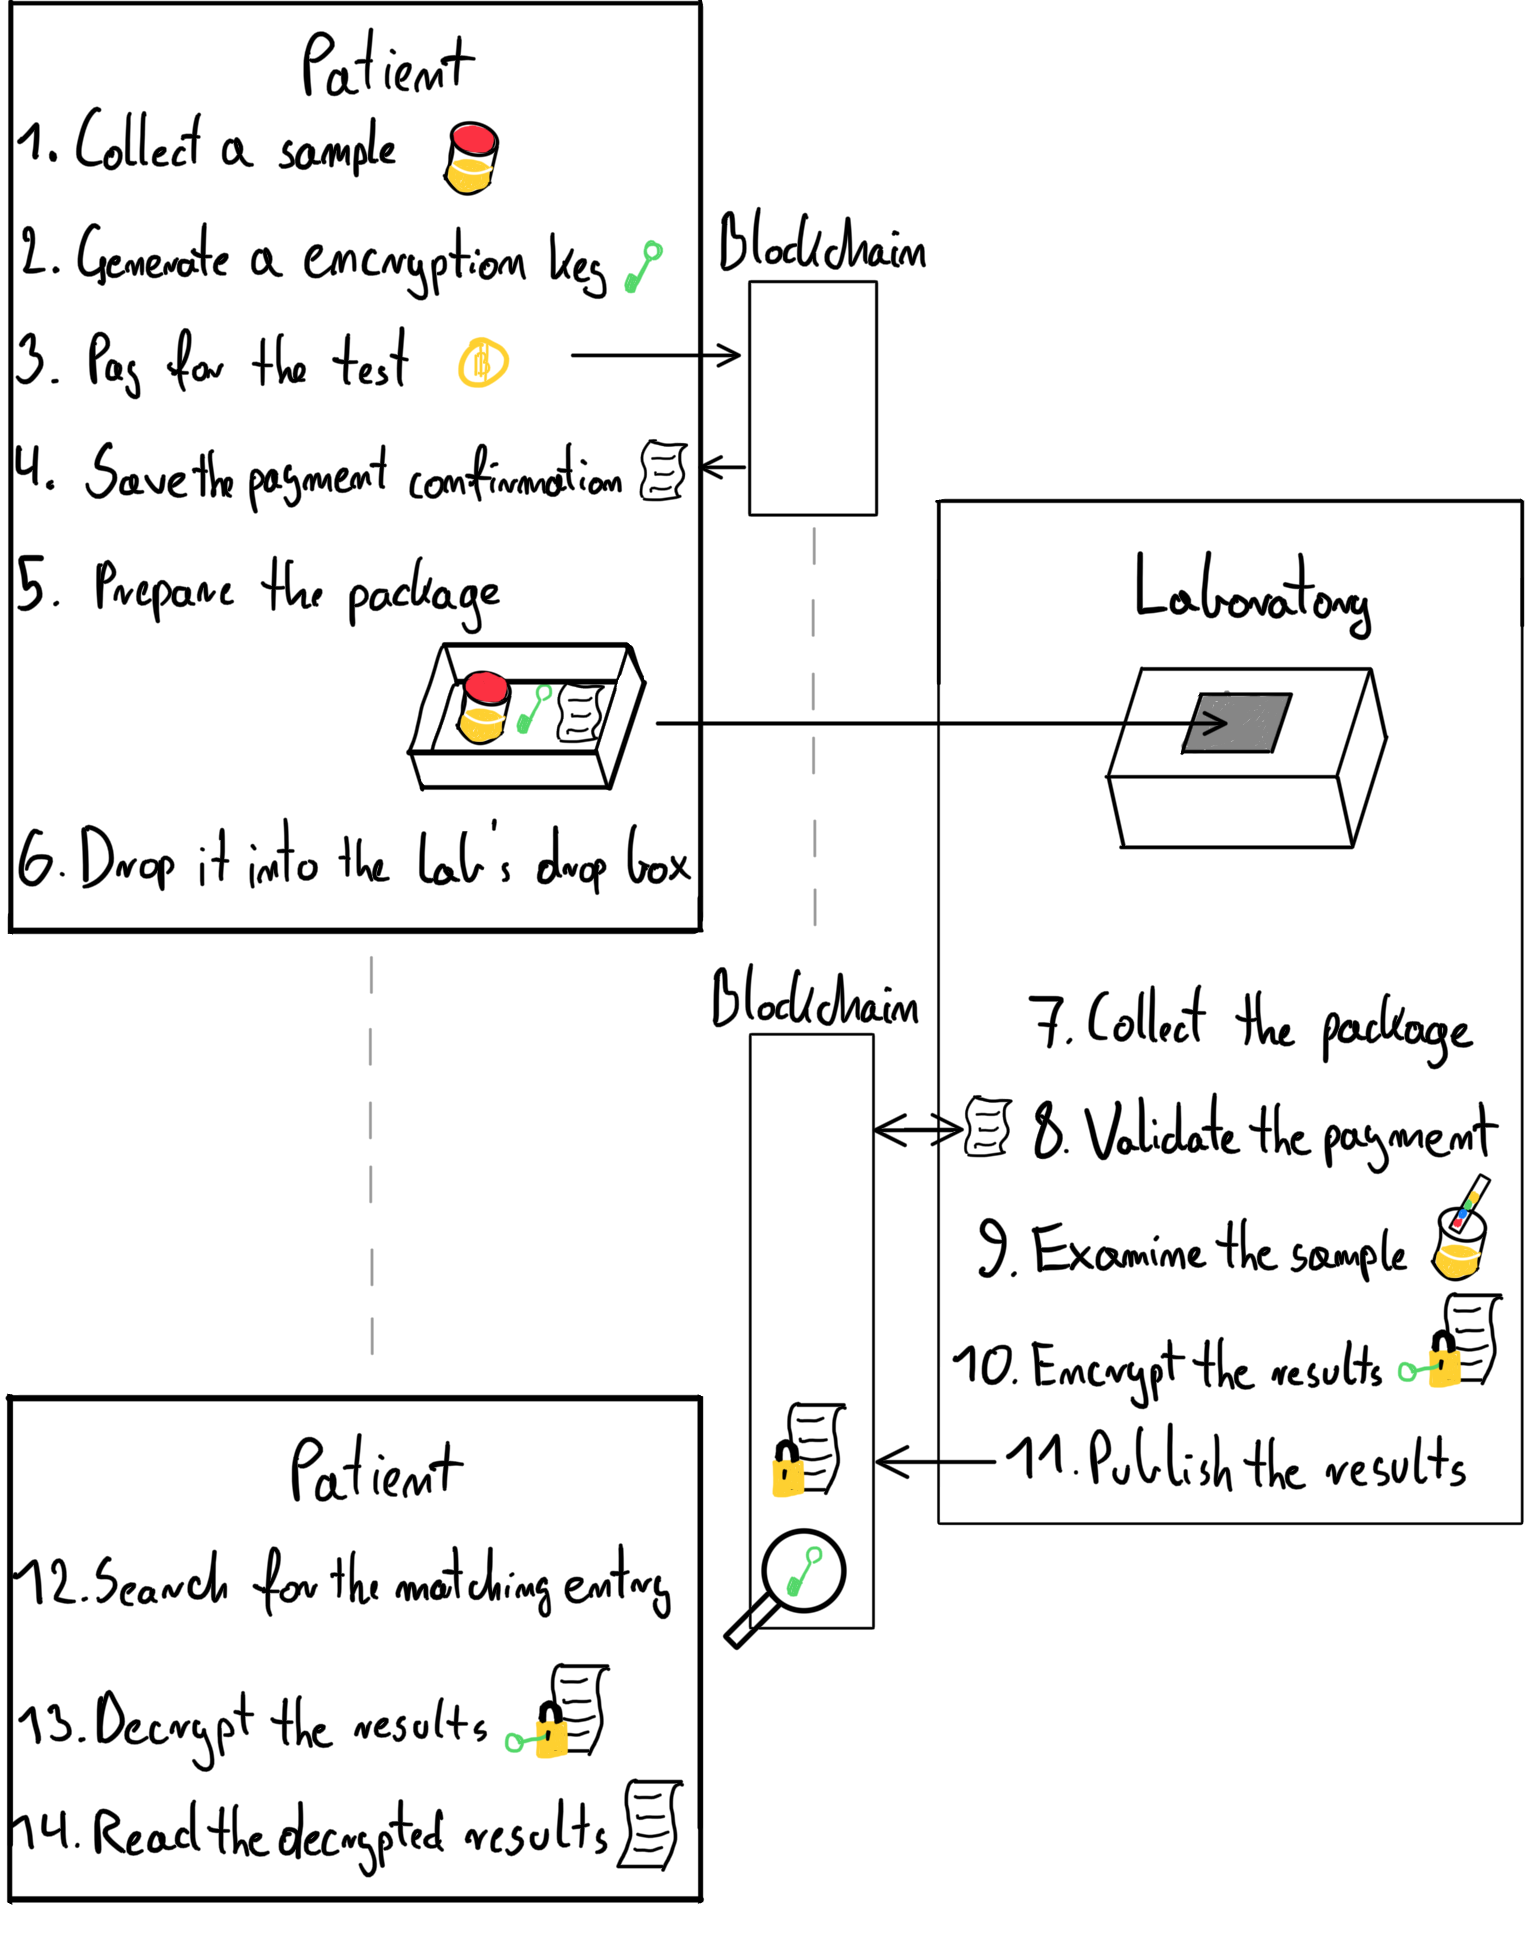
\includegraphics[width=\linewidth]{sequence-flow.png}}
\caption{Sequence flow}
\label{fig:sequence-flow}
\end{figure}

\section{Solution protocol}




\section{Blockchains}
\paragraph{Monero}
Monero offers out-of-the-box proving/checking confidental transactions. \href{https://www.getmonero.org/resources/user-guides/prove-payment.html}

\paragraph{ZCash}
ZCash offers payment disclosure as a preview feature.
\href{https://garethtdavies.medium.com/an-introduction-to-payment-disclosure-in-zcash-96748c209d49}

\href{https://garethtdavies.medium.com/an-introduction-to-payment-disclosure-in-zcash-96748c209d49}

\paragraph{Aleo}

\section{Future work}

Verifiable Document Redacting ~\cite{chabanne2017verifiable} is a protocol for erasing confidential information from authenticated images in verifiable manner. In other words, the protocol allows verifying that only the fields that cover personal information has been blacked out from the authenticated image. This allows users to provide required images without exposing their personal information, and SPs to authenticate the modified images, such that they are sure that only the stated fields have been blacked out and nothing else was touched. 

If such Verifiable Redacted Documents were accepted by other service providers like bank or tax office, national register of the judiciary, then the SP could use the documents provided by the customer to provide wider range of services, without knowing identity of the customer.


% In this paper we extend the idea to a whole user-to-service-provider protocol


\bibliographystyle{alpha}
\bibliography{bibliography}

\end{document}
